\noindent
\textbf{Thermodynamics:
\ifthenelse{\equal{\solutions}{true}}{Examples}{Homework} for chapter 2.}\\

\begin{enumerate}

\item Metallic sodium reacts with water according to:

$$2\textnormal{Na} + \textnormal{H}_2\textnormal{O} \rightarrow 2\textnormal{NaOH} + \textnormal{H}_2$$

If a mole of sodium metal is added to water, how much work is done on the atmosphere (i.e., open beaker; reversible process) by the subsequent reaction if the temperature is constant at 25 $^\circ$C? Assume that H$_2$ is an ideal gas.

\ifthenelse{\equal{\solutions}{true}}{% Problem 1/2 solution
\noindent
\underline{Solution:}\\

First we check that the wavefunctions are normalized. For hydrogenlike atom orbitals we have the following orthonormality condition: $\left<\psi_{n,l,m}\left|\psi_{n',l',m'}\right.\right> = \delta_{nn'}\delta_{ll'}\delta_{mm'}$. The normalization of the given wavefunction can now be evaluated:
\begin{eqnarray}
\nonumber
& & \left<\psi\left|\psi\right.\right> = \frac{1}{14}\left<2\psi_{1,0,0} - 3\psi_{2,0,0} - \psi_{3,2,2}\left|2\psi_{1,0,0} - 3\psi_{2,0,0} - \psi_{3,2,2}\right.\right>\\
\nonumber
& & = \frac{1}{14}(4 + 9 + 1) = 1\textnormal{ (due to orthonormality)}
\end{eqnarray}

\begin{enumerate}
\item The probabilities for the energy eigenstates are given by squaring their coefficients in the wavefunction. The probabilities are then: $P(1,0,0) = 4/14 = 2 / 7, P(2,0,0) = 9/14$ and $P(3,2,2) = 1/ 14$.
\item The expectation value for energy is:
\begin{eqnarray}
\nonumber
& & \left<\psi\left|\hat{H}\right|\psi\right> = \frac{1}{14}\left<2\psi_{1,0,0} - 3\psi_{2,0,0} - \psi_{3,2,2}\left|\hat{H}\right|2\psi_{1,0,0} - 3\psi_{2,0,0} - \psi_{3,2,2}\right>\\
\nonumber
& & = \frac{1}{14}\left(4\overbrace{\left<\psi_{1,0,0}\left|\hat{H}\right|\psi_{1,0,0}\right>}^{=E_{1,0,0}} + 9\overbrace{\left<\psi_{2,0,0}\left|\hat{H}\right|\psi_{2,0,0}\right>}^{= E_{2,0,0}} + \overbrace{\left<\psi_{3,2,2}\left|\hat{H}\right|\psi_{3,2,2}\right>}^{=E_{3,2,2}}\right)\\
\nonumber
& & = \frac{2}{7}E_{1,0,0} + \frac{9}{14}E_{2,0,0} + \frac{1}{14}E_{3,2,2}
\end{eqnarray}

The numerical values for $E_{n,l,m}$'s can be calculated from:
$$E_n = -\frac{hcR}{n^2} = \frac{-13.6\textnormal{ eV}}{n^2} = \frac{E_1}{n^2}$$

Thus the numerical value for $\left<\hat{H}\right>$ is:
$$\left<\hat{H}\right> = \left(\frac{2}{7} + \frac{9}{14}\times\frac{1}{4} + \frac{1}{14}\times\frac{1}{9}\right)E_1 = \frac{229}{504}E_1\approx -6.2\textnormal{ eV}$$

The expectation value for $\vec{\hat{L}}^2$ is:
\begin{eqnarray}
\nonumber
& & \vec{\hat{L}}^2\left|\psi_{n,l,m}\right> = l(l + 1)\hbar^2\left|\psi_{n,l,m}\right>\\
\nonumber
& & \left<\vec{\hat{L}}^2\right> = \frac{\hbar^2}{14}\left(0 + 0 + 2(2 + 1))\right) = \frac{3}{7}\hbar^2
\end{eqnarray}

The expectation value for $\hat{L}_z$ is:
\begin{eqnarray}
\nonumber
& & \hat{L}_z\left|\psi_{n,l,m}\right> = m\hbar\left|\psi_{n,l,m}\right>\\
\nonumber
& & \left<\hat{L}_z\right> = \frac{\hbar}{14}(0 + 0 + 2) = \frac{1}{7}\hbar
\end{eqnarray}

\end{enumerate}

\hrule\vspace{0.5cm}
}{}

\item Show that the differential $d$f is inexact ($a,b,c$ are constants).

$$df = \left(2ax^2 + bxy\right)dx + \left(bx^2 + 2cxy\right)dy$$

Does the corresponding line integral depend on the path? Furthermore, show that differential $df / x$ is exact.

\ifthenelse{\equal{\solutions}{true}}{% Problem 2/2 solution
\noindent
\underline{Solution:}\\

The Hamiltonian consists of the kinetic energy part, which is proportional to the Laplacian operator, and the Coulomb potential.
Laplacian in spherical coordinates is (see lecture notes or a tablebook):

$$\Delta\equiv \nabla^2 = \frac{1}{r^2}\frac{\partial}{\partial r}\left(r^2\frac{\partial}{\partial r}\right) + \frac{1}{r^2\sin(\theta)}\frac{\partial}{\partial\theta}\left(\sin(\theta)\frac{\partial}{\partial\theta}\right)
+ \frac{1}{r^2\sin^2(\theta)}\frac{\partial^2}{\partial\phi^2}$$

The Coulomb potential depends on only on spatial coordinate $r$ (e.g. the distance between the nucleus and the electron). The $\hat{L}_z$ operator is defined in spherical coordinates as:

$$\hat{L}_z = -i\hbar\frac{\partial}{\partial\phi}$$

This clearly commutes with the first two terms in the Laplacian because those terms do not depend on $\phi$. The third depends on $\phi$ but both operators consist of differentiation with respect to $\phi$ and hence they commute. Thus $\left[\hat{H},\hat{L}_z\right] = 0$.

Next we consider $\vec{\hat{L}}^2$. This is operator can be written in spherical coordinates as:
$$\vec{\hat{L}}^2 = -\hbar^2\left[\frac{1}{\sin(\theta)}\frac{\partial}{\partial\theta}\left(\sin(\theta)\frac{\partial}{\partial\theta}\right) + \frac{1}{\sin^2(\theta)}\frac{\partial^2}{\partial\phi^2}\right]$$

This does not depend on $r$ and therefore it commutes with the Coulomb potential and the first term in the Laplacian, which depends only on $r$. Apart from $r$ and some constants $\vec{\hat{L}}^2$ is identical to the angular part of the Laplacian. Operators always commute with themselves. Thus $\left[\hat{H},\vec{\hat{L}}^2\right]$. The significance of these results is that both the energy and the quantum numbers $l$ and $m_l$ can be specified simultaneously.

\hrule\vspace{0.5cm}
}{}

\item Show that the following differential is inexact:

$$df = \left(y^2 - xy\right)dx - x^2dy$$

Test the integrating factor $\frac{1}{xy^2}$ to see if it produces an exact differential.

\ifthenelse{\equal{\solutions}{true}}{% Problem 3/2 solution
\noindent
\underline{Solution:}\\

$$M = y^2 -xy\textnormal{ and }N = -x^2$$

$$\left(\frac{\partial M}{\partial y}\right)_x = 2y - x\textnormal{ and }\left(\frac{\partial N}{\partial x}\right)_y = -2x$$

Because the partial derivatives are not equal, the differential is inexact. If we divide the differential by $xy^2$, we have:

$$M = \frac{1}{x} - \frac{1}{y}\textnormal{ and }N = -\frac{x}{y^2}$$

$$\left(\frac{\partial M}{\partial y}\right)_x = \frac{1}{y^2}\textnormal{ and }\left(\frac{\partial N}{\partial x}\right)_y = -\frac{1}{y^2}$$

and hence differential $\frac{df}{xy^2}$ is inexact (difference in sign only!).

\hrule\vspace{0.5cm}
}{}

\item The state of monoatomic ideal gas ($n = 1$ mol) is changed reversibly as follows:

$$1 \mathop\rightarrow\limits^{\textnormal{A}} 2 \mathop\rightarrow\limits^{\textnormal{B}} 3 \mathop\rightarrow\limits^{\textnormal{C}} 1$$

where 1, 2, 3 and 4 refer to states and A, B and C to processes. Process A is isothermal, B is isobaric and C is isochoric. The cycle is described by the attached graph.

\begin{figure}[htp!]
\centering
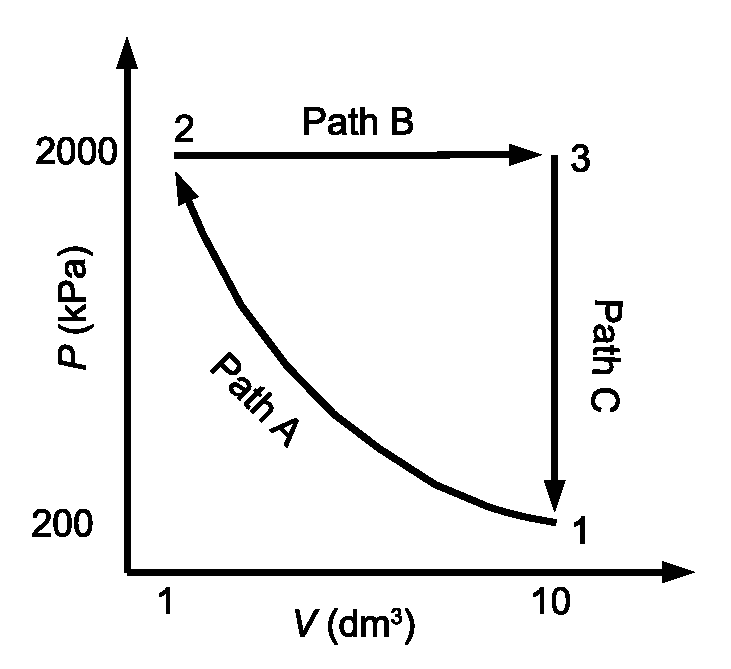
\includegraphics[scale=0.6]{graph}
\end{figure}

What are $\Delta U$, $\Delta H$, $q$ and $w$ after each process (A, B, C), temperatures at points 1, 2, 3,
and $w$ for the whole cycle? Note that for an ideal gas we have: $\bar{U} = \frac{3}{2}RT$ and $\bar{H} = \frac{5}{2}RT$.

\ifthenelse{\equal{\solutions}{true}}{% Problem 4/2 solution
\noindent
\underline{Solution:}\\

\begin{enumerate}

\item \underline{Isothermal process A.} Temperature after A, denoted by $T_2$, is given by the ideal gas law:

$$T_2 = \frac{P_2V_2}{nR} = \frac{(2000\times 10^3\textnormal{ N m}^{-2})(10^{-3}\textnormal{ m}^3)}{(1\textnormal{ mol})(8.314\textnormal{ N m mol}^{-1}\textnormal{ K}^{-1})} = 240.6\textnormal{ K}$$

Both $U$ and $H$ depend only on temperature for ideal gases. This is an isothermal process and hence both $\Delta U$ and $\Delta H$ are zero. The $PV$-work in this step is given by (see lecture notes):

$$w_{rev} = -nRT\ln\left(\frac{V_2}{V_1}\right)$$
$$ = -\left(1\textnormal{ mol}\right)\times\left(8.314\textnormal{ J mol}^{-1}\textnormal{ K}^{-1}\right)\times\left(240.6\textnormal{ K}\right)\times\ln\left(\frac{1\textnormal{ dm}^3}{10\textnormal{ dm}^3}\right) = 4.6\textnormal{ kJ}$$

According to the first law of thermodynamics:

$$\Delta U = q + w \Rightarrow q = \Delta U - w = 0 - 4.6\textnormal{ kJ} = -4.6\textnormal{ kJ}$$

\item \underline{Isobaric process B.} The temperature at 3 is given by the ideal gas law:

$$T_3 = \frac{P_3V_3}{nR} = \frac{(2000\times10^3\textnormal{ N m}^{-2})(10^{-2}\textnormal{ m}^3)}{(1\textnormal{ mol})(8.314\textnormal{ N m mol}^{-1}\textnormal{ K}^{-1})} = 2406\textnormal{ K}$$

Changes in the internal energy and enthalpy are given by:

$$\Delta U = \frac{3}{2}nR\Delta T = \frac{3}{2}nR\left(T_3 - T_2\right)$$
$$ = 1.5 \times (1\textnormal{ mol}) \times\left( 8.314\textnormal{ J mol}^{-1}\textnormal{ K}^{-1}\right) \times \left( 2406\textnormal{ K} - 240.6\textnormal{ K} \right) = 27.0\textnormal{ kJ}$$
$$\Delta H = \frac{5}{2}nR\Delta T = 45.0\textnormal{ kJ}$$

The first law states: $\Delta U = q + w$ and thus if we know either $q$ or $w$, we can always calculate the other. In the isobaric case the work can be obtained with $P_{ext} = P$ and $dw = -P dV$. Integration of this equation gives: $w = -P\Delta V = -(2000 \times 10^3\textnormal{ Nm}^{-2}) \times (10 \times 10^{-3}\textnormal{ m}^3 - 1.0 \times 10^{-3}\textnormal{ m}^3) = -18.0\textnormal{ kJ}$. And further $q = 27.0\textnormal{ kJ} - (-18.0\textnormal{ kJ}) = 45.0\textnormal{ kJ}$.

\item \underline{Isochoric process C.} The temperature at point 1 is given by the ideal gas law:

$$T_1 = \frac{P_1V_1}{nR} = 240.6\textnormal{ K}$$

Changes in the internal energy and enthalpy are given by:

$$\Delta U = \frac{3}{2}nR\Delta T = 1.5\times \left(1\textnormal{ mol}\right) \times \left( 8.314\textnormal{ J mol}^{-1}\textnormal{ K}^{-1}\right)$$
$$\times\left(240.6\textnormal{ K} - 2406\textnormal{ K}\right) = -27.0\textnormal{ kJ}$$

$$\Delta H = \frac{5}{2}nR\Delta T = 2.5\times \left(1\textnormal{ mol}\right) \times \left( 8.314\textnormal{ J mol}^{-1}\textnormal{ K}^{-1}\right)$$
$$\times\left(240.6\textnormal{ K} - 2406\textnormal{ K}\right) = -45.0\textnormal{ kJ}$$

The volume is constant and hence $w = 0$ kJ. The first law gives $q = -27.0$ kJ. The total work in the cycle is: $w_{tot} = w_{\textnormal{A}} + w_{\textnormal{B}} + w_{\textnormal{C}} = (4.61 - 18.0 + 0.00)\textnormal{ kJ} = -13.4\textnormal{ kJ}$.

\end{enumerate}

\hrule\vspace{0.5cm}
}{}

\item One mole of nitrogen (ideal gas) at 25 $^\circ$C and 1 bar is expanded reversibly and isothermally to a pressure of 0.132 bar. (a) What is the value of $w$? (b) What is the value of $w$ if the nitrogen is expanded against a constant external pressure of 0.132 bar?

\ifthenelse{\equal{\solutions}{true}}{% Problem 5/2 solution
\noindent
\underline{Solution:}\\

\begin{itemize}
\item[a)] Based on the lecture notes, we have:

$$w = RT\ln\left(\frac{P_2}{P_1}\right) = \left(8.314\textnormal{ J K}^{-1}\textnormal{ mol}^{-1}\right)\times\left(298.15\textnormal{ K}\right)\times\ln\left(\frac{0.132\textnormal{ bar}}{1\textnormal{ bar}}\right)$$
$$ = -5.03\textnormal{ kJ mol}^{-1}$$

\item[b)] In (a) the pressure changes during the process. Here the external pressure is constant and we can directly calculate:

$$w = -P_{ext}\Delta V = -P_{ext}\left(V_2 - V_1\right)$$
$$V_1 = \frac{nRT}{P_1} = 0.0248\textnormal{ m}^3\textnormal{ and }V_2 = 0.188\textnormal{ m}^3$$

$$\Rightarrow w = -\left(0.132\times 10^5\textnormal{ N m}^{-2}\right)\left(0.188\textnormal{ m}^3 - 0.0248\textnormal{ m}^3\right) = -2.15\textnormal{ kJ mol}^{-1}$$

\end{itemize}

\hrule\vspace{0.5cm}
}{}

\item \begin{itemize}

\item[(a)] Derive the equation for the work of reversible isothermal expansion of a van der Waals gas from $V_1$ to $V_2$.

\item[(b)] A mole of CH$_4$ expands reversibly from 1 to 50 L at 25 $^\circ$C. Calculate the work (in joules) assuming that the gas is ideal.

\item[(c)] A mole of CH$_4$ expands reversibly from 1 to 50 L at 25 $^\circ$C. Calculate the work (in joules) assuming that the gas obeys the van der Waals equation. For CH$_4(g)$, $a$ = 2.283 L$^2$ bar mol$^{-2}$ and $b$ = 0.04278 L mol$^{-1}$.

\end{itemize}

\ifthenelse{\equal{\solutions}{true}}{% Problem 6/2 solution
\noindent
\underline{Solution:}\\

\begin{enumerate}
\item In $^1D_2$ state there are no unpaired electrons (singlet state) and hence the total spin $S = 0$. The angular momentum quantum number $L = 2$, which means that the total angular momentum $\left<\vec{\hat{L}}^2\right> = 2(2 + 1)\hbar^2 = 6\hbar^2$. The total angular momentum quantum number $J = 2$ (specified by the subscript). In $^3F_4$ state the multiplicity ($2S+1$) is 3 which gives $S = 1$ (triplet state) and $F$ term implies $L = 3$. The total angular momentum quantum number is specified as $J = 4$.
\item The energy level diagram for alkai metal atoms is:

\begin{figure}[htp!]
\centering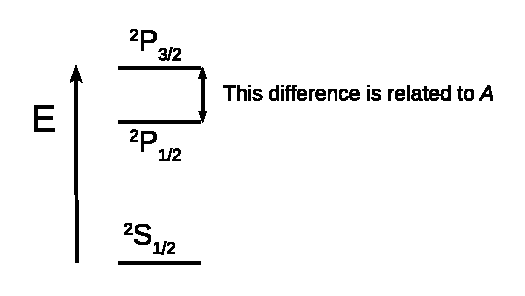
\includegraphics[scale=0.7]{diagram}
\end{figure}

The two emission lines originate from the two $^2P$ states, which are split by the spin-orbit interaction, and terminate to the ground $^2S$ state.
Hence the energy difference between the two emission lines gives the energy difference between the spin-orbit split states $^2P_{1/2}$ and $^2P_{3/2}$.
The line positions must be converted to energy by relation $E = h\nu = \frac{hc}{\lambda}$ ($h$ is the Planck's constant and $c$ is the speed of light).
To calculate $A$, we have to calculate the energy difference between $^2P_{1/2}$ and $^2P_{3/2}$:
\begin{eqnarray}
\nonumber
& & ^2P_{1/2}\textnormal{: }E_{SO} = \frac{A}{2}\left[J(J+1) - L(L+1) - S(S+1)\right] = -A\\
\nonumber
& & ^2P_{3/2}\textnormal{: }E_{SO} = \frac{A}{2}\left[J(J+1) - L(L+1) - S(S+1)\right] = \frac{1}{2}A\\
\nonumber
& & \Delta E_{SO} = \frac{3}{2}A
\end{eqnarray}

Next we calculate the energies for the observed transitions. For $^2P_{3/2}\rightarrow ^2S_{1/2}$ we have:
\begin{eqnarray}
\nonumber
& & E_1 = h\nu_1 = hc / \lambda_1 = (6.6261\times 10^{-34}\textnormal{ Js})\times\frac{2.9979\times 10^8\textnormal{m/s}}{766.70\times 10^{-9}\textnormal{ m}}\\
\nonumber
& &  = 2.5909\times 10^{-19}\textnormal{ J} = 1.6171\textnormal{ eV} = 13043\textnormal{ cm}^{-1}
\end{eqnarray}

For $^2P_{1/2}\rightarrow ^2S_{1/2}$:

\begin{eqnarray}
\nonumber
& & E_2 = h\nu_2 = hc / \lambda_2 = (6.6261\times 10^{-34}\textnormal{ Js})\times\frac{2.9979\times 10^8\textnormal{m/s}}{770.11\times 10^{-9}\textnormal{ m}}\\
\nonumber
& &  = 2.5794\times 10^{-19}\textnormal{ J} = 1.6099\textnormal{ eV} = 12985\textnormal{ cm}^{-1}
\end{eqnarray}

Thus the energy difference is $\Delta E_{SO} = 39$ cm$^{-1}$ which gives $A = 2\Delta E_{SO} / 3 = 39$ cm$^{-1}$.

\item The selection rule is $\Delta l = \pm 1$. For $5d\rightarrow 2s$ we have $\Delta l = -2$ and hence it is forbidden. Transition $5p\rightarrow 3s$ has $\Delta l = -1$ and therefore it is allowed. $5p\rightarrow 3f$ has $\Delta l = +2$ and it is forbidden.

\end{enumerate}

\hrule\vspace{0.5cm}
}{}

\item Liquid water is vaporized at 10 $^\circ$C and 1.013 bar in an open container (reversible process). The heat of vaporization is 40.69 kJ mol$^{-1}$. Assume that water vapor behaves like an ideal gas. What are the values of (a) $w_{rev}$ per mole? (b) $q$ per mole? (c) $\Delta \bar{U}$? (d) $\Delta \bar{H}$?

\ifthenelse{\equal{\solutions}{true}}{% Problem 7/2 solution
\noindent
\underline{Solution:}\\

\begin{enumerate}
\item Consider $2s^12p^1$ electron configuration. The $s$-shell has $l_1 = 0$ with $s_1 = 1/2$ and $p$-shell has $l_2 = 1$ and $s_2 = 1/2$.
The total $L = l_1 + l_2, ..., \left|l_1 - l_2\right| = 1$. The total spin $S = s_1 + s_2, ..., \left|s_1 - s_2\right| = 1, 0$. Thus the total $J = L + S, ..., \left|L - S\right|$ can be 2, 1 or 0 (for $L = 1, S = 1$) or 1 ($L = 1, S = 0$). This results in the following term symbols: $^3P_2, ^3P_1, ^3P_0$ and $^1P_1$.

For $2p^13d^1$ we can have the following:

$p$-electron: $l_1 = 1, s_1 = 1/2$.\\
$d$-electron: $l_2 = 2, s_2 = 1/2$.\\

Hence $L = 3,2,1$ and $S = 1,0$. This gives the following total $J$ values:

\begin{itemize}
\item $L = 3$ and $S = 1$ results in $J = 4,3,2$ ($^3F_4$, $^3F_3$ and $^3F_2$ term symbols)
\item $L = 3$ and $S = 0$ results in $J = 3$ ($^1F_3$ term symbol)
\item $L = 2$ and $S = 1$ results in $J = 3,2,1$ ($^3D_3$, $^3D_2$ and $^3D_1$ term symbols)
\item $L = 2$ and $S = 0$ results in $J = 2$ ($^1D_2$ term symbol)
\item $L = 1$ and $S = 1$ results in $J = 2,1,0$ ($^3P_2$, $^3P_1$ and $^3P_0$ term symbols)
\item $L = 1$ and $S = 0$ results in $J = 1$ ($^1P_1$ term symbol)
\end{itemize}

For Ar$4s^23d^{10}4p^5$ we have only one unpaired electron which has $l = 1$ and $s = 1/2$. This gives obviously $L = 1$ and $S = 1/2$ and the
total $J = 3/2$ or $1/2$. Hence the two possible term symbols are $^2P_{3/2}$ and $^2P_{1/2}$.

% TODO: Prepare the table...
\item Carbon has 2 equivalent $p$-electrons: $l_1 = l_2 = 1$ and $s_1 = s_2 = 1/2$. We should tabulate all the possible states - including $M_L = m_{l_1} + m_{l_2}$ and $M_S = m_{s_1} + m_{s_2}$.

\end{enumerate}

\hrule\vspace{0.5cm}
}{}

\item The heat capacities of a gas may be represented by the Shomate equation (see the NIST Chemistry Webbook):

$$\bar{C}_P = \alpha + \beta T + \gamma T^2 + \delta T^3 + \frac{\eta}{T^2}$$

For N$_2$ gas (between 298 K and 6000 K), $\alpha = 26.09200$ J K$^{-1}$ mol$^{-1}$, $\beta = 8.218801\times 10^{-3}$ J K$^{-2}$ mol$^{-1}$, $\gamma = -1.976141\times 10^{-6}$ J K$^{-3}$ mol$^{-1}$, $\delta = 0.159274\times 10^{-9}$ J K$^{-4}$ mol$^{-1}$ and $\eta = 0.044434\times 10^{6}$ J K mol$^{-1}$. How much heat is required to heat one mole of N$_2$ from 300 K to 1000 K?

\ifthenelse{\equal{\solutions}{true}}{% Problem 8/2 solution
\noindent
\underline{Solution:}\\

$$q = \int\limits_{T_1}^{T_2}\bar{C}_PdT = \alpha T_2 + \frac{\beta}{2} T_2^2 + \frac{\gamma}{3} T_2^3 + \frac{\delta}{4} T_2^4 - \frac{\eta}{T_2} - \alpha T_1 - \frac{\beta}{2} T_1^2 - \frac{\gamma}{3} T_1^3 - \frac{\delta}{4} T_1^4 + \frac{\eta}{T_1}$$

When the constants are inserted in the above expression, we get $q = 21.506$ kJ mol$^{-1}$.

\hrule\vspace{0.5cm}
}{}

\item A mole of argon (ideal gas) is allowed to expand adiabatically and reversibly from a pressure of 10 bar and 298.15 K to 1 bar. What is the final temperature and how much work is done on the argon gas?

\ifthenelse{\equal{\solutions}{true}}{% Problem 9/2 solution
\noindent
\underline{Solution:}\\

Recall the following equations from the lecture notes:

$$\frac{T_2}{T_1} = \left(\frac{P_2}{P_1}\right)^{(\gamma - 1)/\gamma}\textnormal{ where }\gamma = \frac{\bar{C}_P}{\bar{C}_V}$$

For an ideal gas we have:

$$\bar{C}_V = \frac{3}{2}R\textnormal{ and }\bar{C}_P = \frac{5}{2}R \Rightarrow \gamma = 5/3$$

Now we can solve for $T_2$:

$$T_2 = T_1 \left(\frac{P_2}{P_1}\right)^{(\gamma - 1)/\gamma} = (298.15\textnormal{ K})\left(\frac{1.0000\textnormal{ bar}}{10.000\textnormal{ bar}}\right)^{2/5} = 118.70\textnormal{ K}$$

The process is adiabatic which means that $q = 0$. The first law then gives $\Delta U = w$. Since $\left(\frac{\partial U}{\partial V}\right)_T = 0$ for ideal gases, we have:

$$dU = \left(\frac{\partial U}{\partial T}\right)_V dT = C_VdT$$
$$\Rightarrow w = \Delta U = \int\limits_{T_1}^{T_2} C_VdT = \frac{3}{2}R\left(T_2 - T_1\right)$$
$$= \frac{3}{2}\times\left(8.314\textnormal{ J K}^{-1}\textnormal{ mol}^{-1}\right)\times\left(118.70\textnormal{ K} - 298.15\textnormal{ K}\right) = -2238\textnormal{ J mol}^{-1}$$

\hrule\vspace{0.5cm}
}{}

\item Calculate $\Delta_rH^\circ$ at 298 K for:

$$\textnormal{H}_2(g) + \textnormal{F}_2(g) \rightarrow 2\textnormal{HF}(g)$$
$$\textnormal{H}_2(g) + \textnormal{Cl}_2(g) \rightarrow 2\textnormal{HCl}(g)$$
$$\textnormal{H}_2(g) + \textnormal{Br}_2(g) \rightarrow 2\textnormal{HBr}(g)$$
$$\textnormal{H}_2(g) + \textnormal{I}_2(g) \rightarrow 2\textnormal{HI}(g)$$

Use the data available in the NIST Chemistry Webbook\\
(http://webbook.nist.gov/chemistry/).

\ifthenelse{\equal{\solutions}{true}}{% Problem 10/2 solution
\noindent
\underline{Solution:}\\

We use the following equation (see lecture notes):

$$\Delta_r H^\circ = \sum\limits_{i=1}^{N_s}v_i\Delta_fH_i^\circ$$

By looking up the data from the table and using this equation, we get:

$$2 \times (-273.30\textnormal{ kJ mol}^{-1}) - (0\textnormal{ kJ mol}^{-1}) - (0\textnormal{ kJ mol}^{-1})= -546.60\textnormal{ kJ mol}^{-1}$$
$$2 \times (-92.31\textnormal{ kJ mol}^{-1}) - (0\textnormal{ kJ mol}^{-1}) - (0\textnormal{ kJ mol}^{-1}) = -184.62\textnormal{ kJ mol}^{-1}$$
$$2 \times (-36.29\textnormal{ kJ mol}^{-1}) - (30.91\textnormal{ kJ mol}^{-1}) - (0\textnormal{ kJ mol}^{-1}) = -103.49\textnormal{ kJ mol}^{-1}$$
$$2 \times (26.50\textnormal{ kJ mol}^{-1}) - (62.42\textnormal{ kJ mol}^{-1}) - (0\textnormal{ kJ mol}^{-1}) = -9.42\textnormal{ kJ mol}^{-1}$$

\hrule\vspace{0.5cm}
}{}

\item One gram of liquid benzene is burned in an adiabatic bomb calorimeter. The temperature before ignition was 20.826 $^\circ$C, and the temperature after the combustion was 25.000 $^\circ$C. The heat capacity of the bomb, the water around it, and the contents of the bomb before the combustion was 10 000 J K$^{-1}$. Calculate $\Delta_fH^\circ$ for C$_6$H$_6(l)$ at 298.15 K from these data. Assume that the water produced in the combustion is in the liquid state, the carbon dioxide produced in the combustion is in the gas state and all gases
behave according to the ideal gas law. The combustion reaction is:

$$2\textnormal{C}_6\textnormal{H}_6(l) + 15\textnormal{O}_2(g) \rightarrow 12\textnormal{CO}_2(g) + 6\textnormal{H}_2\textnormal{O}(l)$$

\ifthenelse{\equal{\solutions}{true}}{% Problem 11/2 solution
\noindent
\underline{Solution:}\\

Even though this is called adiabatic, there is heat exchange between the sample (liquid benzene; system) and the surrounding water bath around it. The adiabaticity means that there is no thermal contact between the bath and the rest of the world. The total volume of the system is constant, which means that $w = P\Delta V = 0$ and $\Delta U = q$. Thus the heat released to the bath must correspond to the change in internal energy of the system. The heat capacity of the system+bath was given, so we can relate the temperature increase in
the bath to the amount of heat released from the system:

$$\Delta U = q = -\int\limits_{T_1}^{T_2}C_{\textnormal{system+bath}}dT = -C_{\textnormal{system+bath}}\Delta T$$
$$ = -\left(10\textnormal{ kJ K}^{-1}\right)\times\left(4.174\textnormal{ K}\right) = -41.74\textnormal{ kJ}^{-1}$$

where the minus signifies that heat flows out of the system). Since the molecular weight of benzene is 78 g mol$^{-1}$ and we had 1 gram of benzene, we finally get: $\Delta U = -3255.7$ kJ mol$^{-1}$.

In order to get $\Delta H$ for the reaction, one must consider the fact that gaseous products are consumed/formed. Let's first write the equation in standard form:

$$\textnormal{C}_6\textnormal{H}_6(l) + 7.5\textnormal{O}_2(g) \rightarrow 6\textnormal{CO}_2(g) + 3\textnormal{H}_2\textnormal{O}(l)$$

So we see that when one mole of benzene burns, 7.5 moles of O$_2$ gas is consumed and 6 moles of CO$_2$ is formed. This means that the pressure in the bomb is not constant. Recall that $H = U + PV$ and hence $\Delta H = \Delta U + \Delta (PV) = \Delta U + P\Delta V + V\Delta P$. The volume is constant, so we don't need to consider the $P\Delta V$ term. If we consider that both O$_2$ and CO$_2$ are ideal gases (the total amount of gas is denoted by $n_{gas}$), then we can write $\Delta (PV) = R\Delta (n_{gas}T) = RT\Delta n_{gas} + Rn_{gas}\Delta T \approx RT\Delta n_{gas}$. In this example, $\Delta n = 6.0 - 7.5 = -1.5$. Thus we have ($T = 298$ K):

$$\Delta \bar{H}_{298\textnormal{ K}} = \Delta \bar{U} + \frac{RT\Delta n_{gas}}{1\textnormal{ mol}} = -3255.7\textnormal{ kJ mol}^{-1} - 1.5RT/\textnormal{mol} = -3259.4\textnormal{ kJ mol}^{-1}$$

From the NIST Chemistry Webbook we have the following values: $\Delta H_f(\textnormal{CO}_2(g)) = -393.51\textnormal{ kJ mol}^{-1}$, $\Delta H_f(\textnormal{H}_2\textnormal{O}(l)) = -285.83\textnormal{ kJ mol}^{-1}$ and $\Delta H_f(\textnormal{O}_2(g)) = 0\textnormal{ kJ mol}^{-1}$. If we write the reaction using heats of formation, we have:

$$\Delta H_f(\textnormal{C}_6\textnormal{H}_6(l)) + 7.5 \times \Delta H_f(\textnormal{O}_2(g)) + \Delta H_{298\textnormal{ K}} = 6 \times \Delta H_f(\textnormal{CO}_2(g)) + 3 \times \Delta H_f(\textnormal{H}_2\textnormal{O}(l))$$

Note that the '$-$' sign in $\Delta H_{298\textnormal{ K}}$ signifies that the system (benzene) is loosing energy and hence when we place it in the above equation $\Delta H_{298\textnormal{ K}}$ has a positive sign when it is put on the left hand side and negative when put on the right hand side. On the right hand side it would yield positive number, which states that energy is being released. By solving for $\Delta H_f(\textnormal{C}_6\textnormal{H}_6(l))$ from this equation we get:

$$\Delta H_f(\textnormal{C}_6\textnormal{H}_6(l)) = 6 \times (-393.51\textnormal{ kJ mol}^{-1}) + 3 \times (-285.83\textnormal{ kJ mol}^{-1})$$
$$ - (-3259.4\textnormal{ kJ mol}^{-1}) = 40.9\textnormal{ kJ mol}^{-1}$$

(The literature value is \textit{ca.} 49 kJ mol$^{-1}$ -- not a great measurement accuracy...)

\hrule\vspace{0.5cm}
}{}

\end{enumerate}
